\documentclass[conference]{IEEEtran}
\IEEEoverridecommandlockouts
% The preceding line is only needed to identify funding in the first footnote. If that is unneeded, please comment it out.
\usepackage{cite}
\usepackage{amsmath,amssymb,amsfonts}
\usepackage{algorithmic}
\usepackage{graphicx}
\usepackage{textcomp}
\usepackage{xcolor}
\usepackage{float}
\def\BibTeX{{\rm B\kern-.05em{\sc i\kern-.025em b}\kern-.08em
    T\kern-.1667em\lower.7ex\hbox{E}\kern-.125emX}}
\begin{document}

\title{PostgreSQL Scaling: Analysis of Techniques and Use Case Justification\\
}

\author{\IEEEauthorblockN{Jayraj Kiran Ladkat}
\IEEEauthorblockA{\textit{Department of Computer Engineering and Technology} \\
\textit{Dr. Vishwanath Karad MIT World Peace University}\\
Pune, India \\
jayrajkladkat@gmail.com}
\and
\IEEEauthorblockN{Prof. Pranati Waghodekar}
\IEEEauthorblockA{\textit{Department of Computer Engineering and Technology} \\
\textit{Dr. Vishwanath Karad MIT World Peace University}\\
Pune, India \\
pranati.waghodekar@mitwpu.edu.in}
}

\maketitle

\begin{abstract}
Scalable databases are necessary for large data volumes and heavy query loads in modern applications. Five PostgreSQL scaling strategies—Vertical Scaling, Read Replicas, Partitioning, Custom Sharding, and Connection Pooling—are thoroughly examined in this work. We assess their cost-effectiveness, scalability, complexity, and performance (e.g., delivering 2x-5x throughput improvements, reducing latency by 30-50ms). Our research offers useful information that helps builders choose the best tactics for reliable, efficient, and financially feasible PostgreSQL solutions that can manage hundreds of thousands of connections.
\end{abstract}

\begin{IEEEkeywords}
PostgreSQL, Database Scaling, Performance Analysis, Replication, Data Partitioning, Sharding
\end{IEEEkeywords}

\section{Introduction}
The volume, variety's, and velocity of data have increased at an unprecedented and unaccounted rate in today's data-driven world due to the exponential rise of applications and services.\cite{b4}\cite{b5} Databases must scale effectively to manage heavy loads, guarantee low latency, and preserve dependability in order to satisfy these needs. A crucial component of contemporary application architecture is database scalability, which allows systems to handle expanding user populations and workloads without sacrificing availability or performance. This study examines several database scaling methods and technologies, emphasizing their advantages, disadvantages, and real-world uses.

The paper discusses both more sophisticated techniques like custom sharding and connection pooling as well as more conventional ones like read replicas, partitioning, and vertical scaling\cite{b2}\cite{b2}.\cite{b13}

Each method that is evaluated across key parameters like scalability potential, performance impact, implementation complexity, and cost-effectiveness. While vertical scaling does offers us simplicity by upgrading hardware resources, it is quite inherently limited by physical constraints. Horizontal scaling on the other hand provide us with a methods such as sharding which provide greater scalability but require significant architectural changes. Emerging technologies like Connection Pooling introduce us with intelligent resource management, making them highly effective for dynamic workloads and deployments. 

Through this research, we seek to:
\begin{itemize}
\item Quantify the trade-offs: Provide empirical data and analysis to clearly define the performance, complexity, and cost implications of each scaling technique, moving beyond from the just theoretical discussions.
\item Develop a decision framework: Establish a structured guide or methodology that helps architects and developers choose the optimal scaling strategy tailored to specific application requirements and their workload characteristics.
\item Identify best practices for hybrid approaches: Explore how combinations of these techniques can be leveraged synergistically to achieve superior scalability and resilience for complex, evolving data environments.
\end{itemize}

This comparative analysis aims to provide us with insights into selecting the most appropriate database scaling techniques based on specific application requirements. By understanding the trade-offs between these approaches, organizations can design scalable and efficient systems to meet the challenges of modern data management.

\section{Literature Review}

\subsection{Specific Application Based Review}
\begin{table}[htbp]
\centering
\small
\begin{tabular}{|p{1.7cm}|p{1.9cm}|p{2.1cm}|p{1.9cm}|}
\hline
\textbf{Paper Title} & \textbf{Work Done} & \textbf{Technique} & \textbf{Key Results} \\
\hline
PostgreSQL Database Performance Optimization\cite{b6} & Examined PostgreSQL performance optimization techniques and demonstrated with test cases. & Indexing, configuration tuning, query optimization & Improved query execution, better resource utilization, practical guidance for PostgreSQL DBAs. \\
\hline
PostgreSQL as a Multi-Model Database\cite{b7} & Evaluated PostgreSQL as a multi-model database for various data models (row, column, key-value, document). & Row/column/key-value/document-oriented modeling, extensions & PostgreSQL supports multi-model use cases; row-oriented best for OLTP, column-oriented for OLAP, efficient for unstructured data with JSON/JSONB. \\
\hline
\end{tabular}
\end{table}

\begin{table}[htbp]
\centering
\small
\begin{tabular}{|p{1.6cm}|p{1.8cm}|p{2.0cm}|p{1.8cm}|}
\hline
\textbf{Paper Title} & \textbf{Work Done} & \textbf{Technique} & \textbf{Key Results} \\
\hline
Horizontal v/s Vertical Scaling in Modern Database Systems Landscape: Comparative Analysis of Performance and Cost Trade-Offs to consider\cite{b8} & Comparative analysis of vertical and horizontal scaling in modern databases, including case studies and literature review. & Vertical (scale-up), horizontal (scale-out), hybrid, cloud-native scaling & Vertical scaling is simpler but limited; horizontal scales better but is complex; hybrid and cloud-native solutions offer flexibility.\\
\hline
The Choice of Scaling Technique Matters for Classification Performance\cite{b2} & Compared impact of 5 scaling techniques on 20 classification algorithms. & Dataset scaling (normalization) techniques & Choice of scaling technique significantly affects classification performance, especially for imbalanced datasets.\\
\hline
Measurement and Scaling Techniques in Research Methodology\cite{b10} & Summarized scaling methods for survey/questionnaire research. & Various scaling methods (Likert, Guttman, Thurstone, etc.) & Provided guidelines for selecting appropriate scaling methods in research.\\
\hline
Scaling Automated Database System Testing\cite{b2} & Addressed the challenge of scaling automated DBMS testing by reducing the effort required to adapt test oracles. & SQLancer++, an adaptive SQL statement generator; model-based schema representation; bug-prioritization approach & Discovered 195 unique, previously unknown bugs across 17 DBMSs, with 180 fixed, demonstrating effectiveness and scalability in finding logic bugs.\\
\hline
Database Scaling on Kubernetes\cite{b1} & Investigated scaling databases (including PostgreSQL) in Kubernetes environments, covering autoscaling and high availability. & Kubernetes-based scaling, autoscaling, data synchronization, distributed computing & Demonstrated effective database scaling in Kubernetes, with improved availability, performance, and reduced operational complexity.\\
\hline
\end{tabular}
\end{table}

\begin{table}[htbp]
\centering
\small
\begin{tabular}{|p{1.6cm}|p{1.8cm}|p{2.0cm}|p{1.8cm}|}
\hline
\textbf{Paper Title} & \textbf{Work Done} & \textbf{Technique} & \textbf{Key Results} \\
\hline
A Study of Database Connection Pool in Microservice Architecture\cite{b13} & Studied optimal database connection pool size for backend systems in microservice architectures. & Connection pooling, microservice architecture, load balancing & Found that a pool size of 5 connections provides the best performance and latency results; max latency 53ms, 99th percentile 19ms at 2000 requests/sec. {b13}\\
\hline
Citus: Distributed PostgreSQL for Data-Intensive Applications\cite{b14} & Analyzed requirements of 4 common workload patterns and how Citus distributively addresses them; included benchmarks and architectural insights. & Citus (Distributed PostgreSQL), horizontal scaling, sharding, parallel query execution & Citus effectively scales PostgreSQL for data-intensive workloads, supports parallel queries, and provides robust performance for analytics and multi-tenant applications.\\
\hline
\end{tabular}
\hline
\caption{REVIEW ON EXISTING POSTGRESQL SCALING TECHNIQUES}
\label{tab:postgresql_research_summary}
\end{table}

\subsection{Research Gap}
\begin{itemize}
\item Limited Real-World Benchmarking for Multi-Model PostgreSQL: While PostgreSQL’s multi-model capabilities are explored, there is a lack of comprehensive, real-world benchmarks comparing its performance for different data models (relational, document, graph, vector) under varied workloads and at scale
\item Item Combining Vector Data Processing and Contemporary AI/ML: There is little published research on how well PostgreSQL interacts with sophisticated AI/ML pipelines, particularly for vector-based similarity search and recommendation systems in production contexts, despite the existence of extensions like pgvector and PostgresML. 
\item Trade-offs between Scalability and Performance in Cloud-Native and Kubernetes Environments: The performance and operational trade-offs of vertical vs. horizontal scaling, custom sharding, and connection pooling in cloud-native, distributed PostgreSQL deployments require further investigation, even as Kubernetes-based scaling is examined. 
\item Resource Management and Automated Scaling: The dynamic resource allocation issues and cost optimization techniques for mixed OLTP/OLAP workloads are not adequately covered by the current research on automated scaling (e.g., Citus-based sharding, Kubernetes autoscaling). 
\end{itemize}

\begin{table}[htbp]
\centering
\small
\begin{tabular}{|p{2.4cm}|p{2.4cm}|p{2.4cm}|}
\hline
\textbf{Parameter} & \textbf{Vertical Scaling} & \textbf{Horizontal Scaling} \\
\hline
Definition & Increasing resources (CPU, RAM, storage) on a single server & Adding more servers to distribute the load \\
\hline
Scalability & Limited by hardware constraints of a single node & Virtually unlimited, as more nodes can be added \\
\hline
Complexity & Simpler to implement and manage & More complex; requires distributed architecture, data partitioning, and synchronization \\
\hline
Cost & High initial cost for high-end hardware; may be cost-effective for small workloads & Lower per-node cost; total cost may be higher due to management overhead \\
\hline
Performance & Better for single-threaded or non-distributed workloads & Better for parallel, distributed, or read-heavy workloads \\
\hline
High Availability & Depends on single node; downtime during upgrades or failures & Improved by redundancy and failover across multiple nodes \\
\hline
Maintenance & Easier to maintain, fewer components & More complex maintenance; requires coordination across nodes \\
\hline
Use Case & OLTP, small-to-medium workloads, low concurrency & OLAP, large-scale, high-concurrency, distributed workloads \\
\hline
\end{tabular}
\hline
\caption{COMPARATIVE ANALYSIS: VERTICAL SCALING VS. HORIZONTAL SCALING}
\label{tab:postgresql_research_summary}
\end{table}

\section{Material and Method}
\subsection{AWS PostgreSQL Testing Instance\cite{b17}}\label{AA}
\begin{itemize}
\item \textbf{Engine Version:} PostgreSQL 17.4 is a recent and supported version on AWS RDS. \\
\item \textbf{Instance Class:} db.m7g.large is suitable for development and testing workloads, offering a good balance of compute and memory. \\
\item \textbf{Storage:} 50 GB General Purpose SSD (gp3) is cost-effective for dev/test and provides good performance. \\
\item \textbf{Security:} Always restrict access using security groups and enable encryption for data protection. \\
\item \textbf{Public Accessibility:} Enable only if required for your workflow; for production or sensitive environments, keep it private. \\
\item \textbf{Backup:} Short retention is sufficient for dev/test to minimize costs. \\
\item \textbf{High Availability:} Not required for dev/test, but can be enabled for critical test scenarios. \\
\end{itemize}

\subsection{Vertical Scaling(VS)\cite{b2}\cite{b8}}
Vertical scaling refers to increasing the capacity of a single database server by increasing its hardware resources, such as CPU, memory, and storage or sometimes network. This approach is straightforward and often the first step taken to address performance bottlenecks, as it does not require changes to application code or database architecture. Vertical scaling is particularly useful when workloads are predictable and do not exceed the maximum capabilities of a single server. However, it is limited by the upper bounds of the hardware and may involve brief downtime during upgrades, especially in single-availability-zone deployments. Vertical scaling is commonly used in cloud environments like AWS RDS, where instance classes can be changed with minimal disruption, especially when using Multi-AZ configurations.

\subsection{Read Replica\cite{b19}\cite{b20}}
Read replicas are read-only copies of a primary (master) database that are kept synchronized through asynchronous replication. They allow read-heavy workloads to be distributed across multiple servers and databases, reducing the load on the primary instance of our database and improving overall application performance and availability. Read replicas are particularly valuable in environments with high query volumes, such as analytics dashboards or reporting applications. This approach enables horizontal scaling for read operations and can also enhance disaster recovery by acting as failover targets. Managing read replicas requires careful monitoring to ensure data consistency and to handle replication lag.

\subsection{Partitioning\cite{b22}}
Partitioning is the process of breaking up a large database table into tiny ones, which are easier-to-manage sections known as partitions. Usually, this is done using a key like date, region, or customer ID. This method decreases index size, streamlines data management operations like archiving and deletion, and enhances query performance by restricting the volume of data scanned for each query. Large data sets and analytical workloads benefit greatly from partitioning since it facilitates quicker data retrieval and more effective maintenance procedures. Declarative partitioning is made possible by PostgreSQL's native partitioning features, which simplify the implementation and administration of partitioned tables. 

\subsection{Connection Pooling\cite{b13}}
By managing a cache of database connections, connection pooling enables several clients to share connections rather than establishing new ones for every request. By lowering the overhead involved in creating and breaking connections, this improves throughput, lowers latency, and makes better use of available resources. In high-concurrency settings where frequent database access could otherwise overload the server, like web applications or microservices architectures, connection pooling is crucial. Strong connection pooling options for PostgreSQL are offered by tools such as PgBouncer and integrated application frameworks. 

\subsection{Custom Sharding\cite{b14}\cite{b22}}
Custom sharding is a horizontal scalability technique in which a subset of the data is managed by each shard, which is spread across several database instances or servers. Usually, to accomplish this, queries are routed to the relevant shard according to a sharding key, like user ID or location. For big, high-throughput applications, custom sharding allows for effective scaling and parallel processing. Despite its substantial scalability advantages, it adds complexity to query routing, data dissemination, and transaction management. Sharding is frequently utilized in large-scale applications and distributed systems where read replicas and vertical scalability are not enough. .

\section{Results and Discussions}

\subsection{Base Case Postgres instance with optimization(indexing)}
\begin{figure}[H]
    \centering
    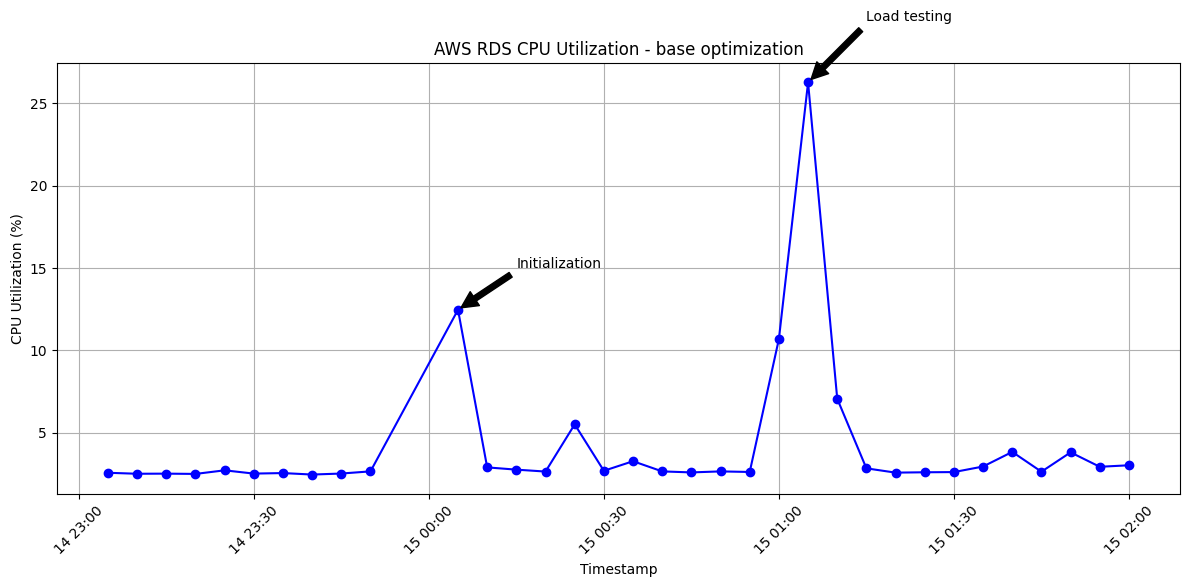
\includegraphics[width=0.75\linewidth]{images/image.png}
    \caption{AWS RDS CPU Utilization over time. The Y-axis shows us CPU Utilization (\%) and the X-axis shows us Timestamp (UTC).}
    \label{fig:cpu_utilization}
\end{figure}

\begin{figure}[H]
    \centering
    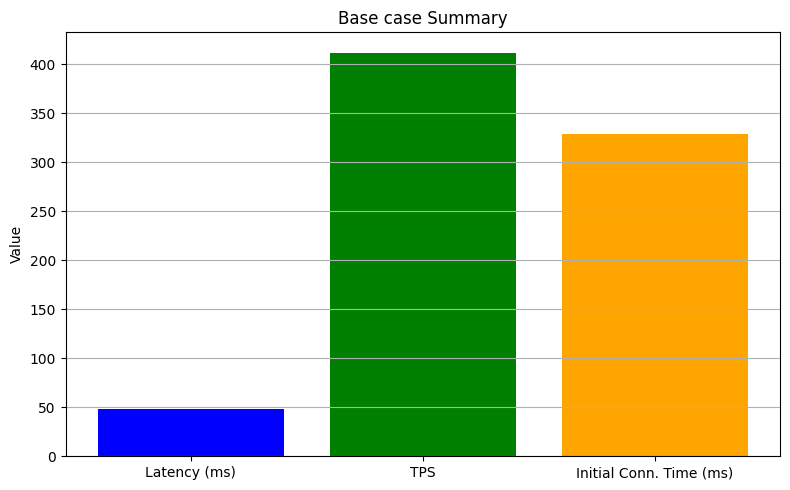
\includegraphics[width=0.75\linewidth]{images/image2.png}
    \caption{Summary of base case Postgres instance performance metrics measured using pgBench benchmarking. Metrics include Latency (ms), Transactions Per Second (TPS), and Initial Connection Time (ms).}
    \label{fig:base_summary}
\end{figure}

\begin{figure}[H]
    \centering
    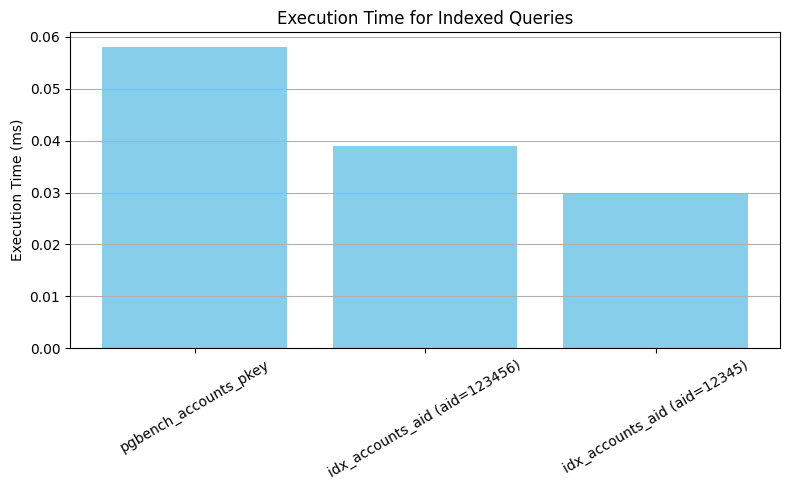
\includegraphics[width=0.75\linewidth]{images/image3.png}
    \caption{Execution time comparison for indexed queries on the pgbench\_accounts table. The X-axis shows Query Type (primary key or secondary indexes) and the Y-axis shows Execution Time (ms).}
    \label{fig:indexed_query_comparison}
\end{figure}


\subsection{Read Replica}
\begin{figure}[H]
    \centering
    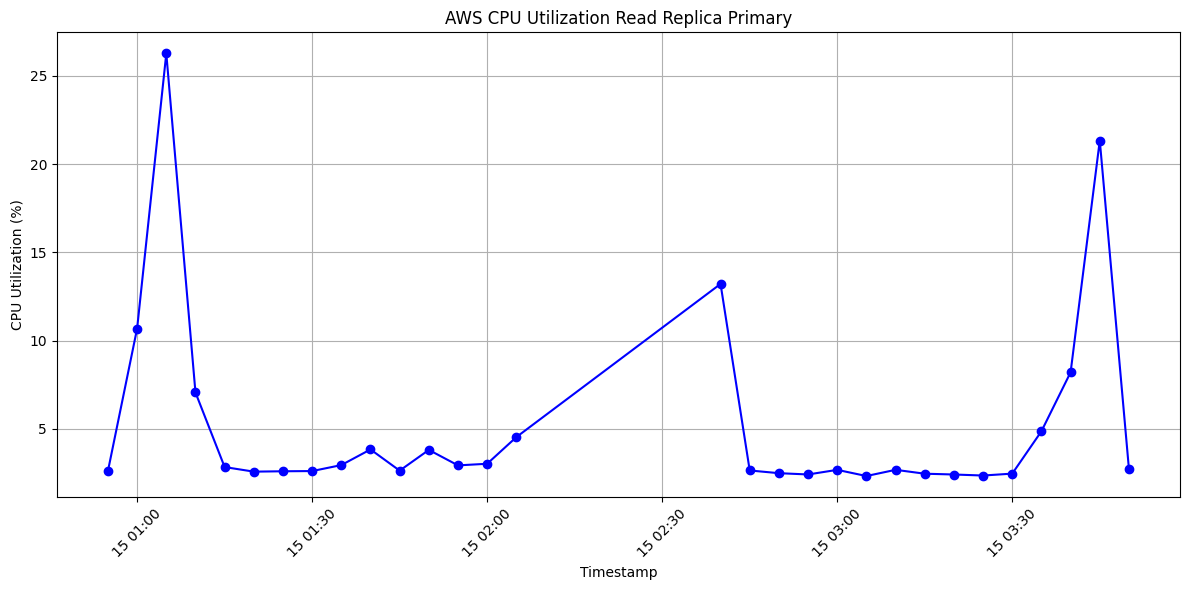
\includegraphics[width=0.75\linewidth]{images/image4.png}
    \caption{CPU Utilization of the AWS RDS Read Replica Primary instance. The graph illustrates significant spikes in CPU usage at around 01:00, 02:30, and 03:45, reaching peaks of over and above 25\%. These spikes may correspond to periods of increased read traffic or maintenance tasks, while the rest of the time shows minimal CPU load, suggesting us overall efficient resource usage during low-load periods.}
    \label{fig:aws_cpu_utilization}
\end{figure}

\begin{figure}[H]
    \centering
    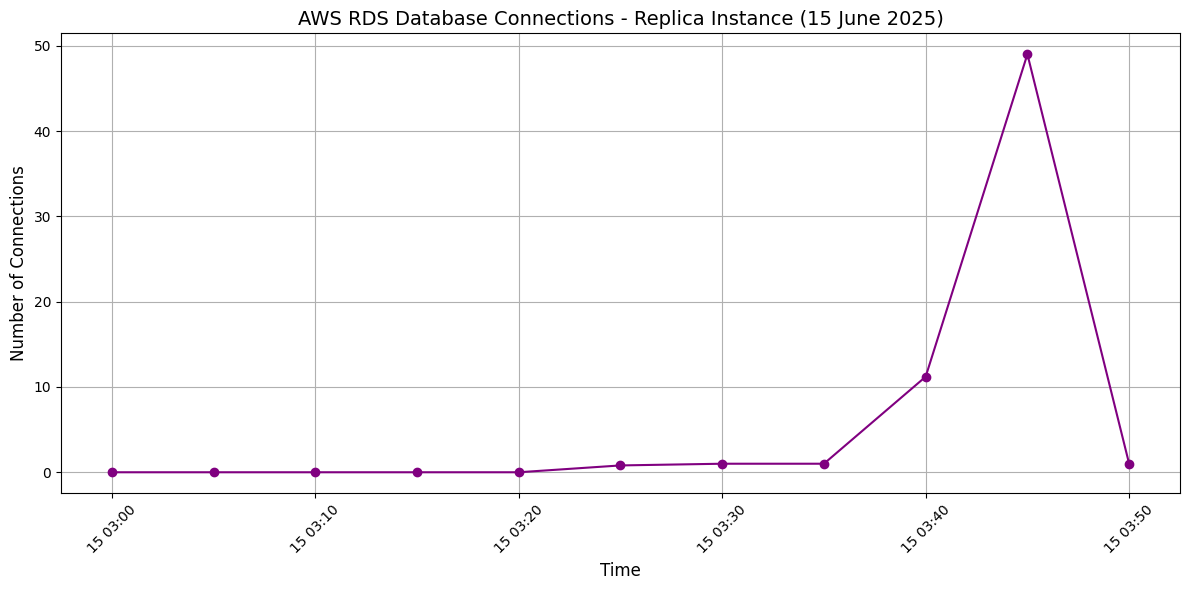
\includegraphics[width=0.75\linewidth]{images/image5.png}
    \caption{Number of database connections to the AWS RDS Read Replica instance. The graph shows a sudden surge in connections starting at 03:40, peaking at nearly 50 active connections before rapidly dropping back to near zero. This behavior indicate us a burst of read operations or automated system queries, providing us insights into usage patterns and potential performance bottlenecks.}
    \label{fig:aws_rds_connections}
\end{figure}

\subsection{Partitioning}

\begin{table}[H]
\centering
\caption{Comparison of Query Performance: Unpartitioned vs. Partitioned Tables}
\begin{tabular}{p{2.4cm}|p{2.4cm}|p{2.4cm}}
\hline
\textbf{Feature/Metric} & \textbf{SELECT * FROM large\_events WHERE event\_time BETWEEN '2023-02-01' AND '2023-02-28' (Unpartitioned)} & \textbf{SELECT * FROM partitioned\_events WHERE event\_time BETWEEN '2023-02-01' AND '2023-02-28' (Partitioned)} \\
\hline
Table Type & Unpartitioned & Partitioned (by event\_time) \\
\hline
Query Plan Root & Gather (then Parallel Seq Scan) & Seq Scan (on a specific partition) \\
\hline
Execution Time & 34.227ms & 0.021ms \\
\hline
Buffers: Shared Hit & 10838 & 1 \\
\hline
Rows Returned & 38881 & 1 \\
\hline
Filter Efficiency & Scans entire table, then filters & Utilizes partition pruning, scanning only relevant partition(s) \\
\hline
Optimization & Parallel Sequential Scan & Partition Pruning \\
\hline
\end{tabular}
\label{tab:partition-comparison}
\end{table}


\subsection{Connection Pooling}
\begin{figure}[H]
    \centering
    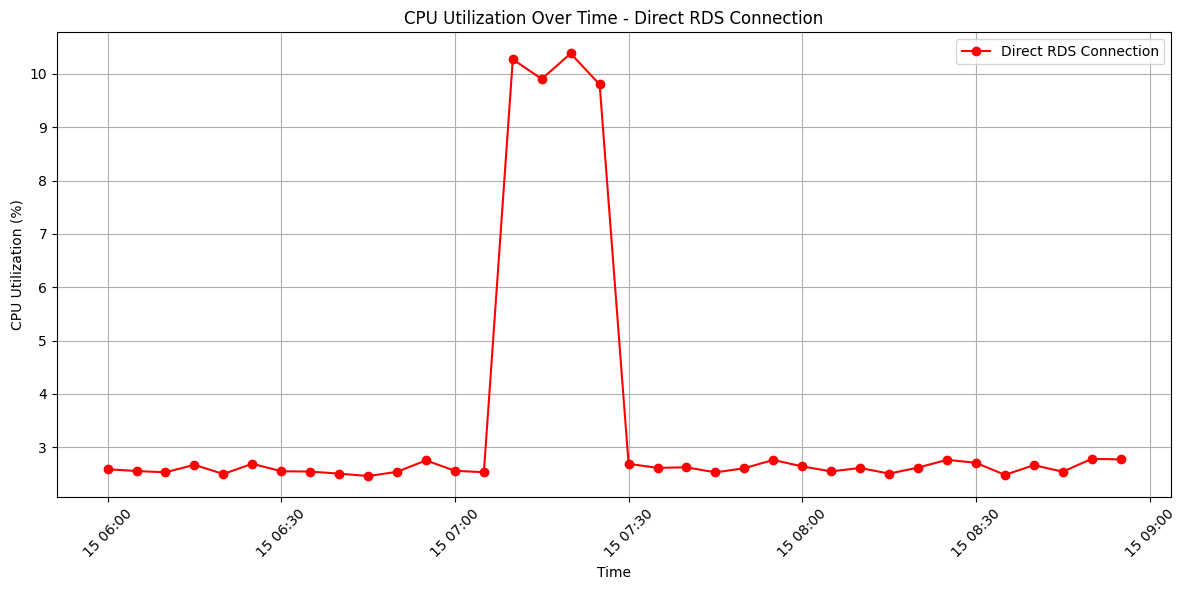
\includegraphics[width=0.75\linewidth]{images/image6.png}
    \caption{CPU Utilization Over Time for Direct RDS Connection. A noticeable spike is observed between 03:07:00 and 03:07:00, indicating a temporary workload surge. Outside this window, CPU usage remains relatively stable around 2.5--2.7\%.}
    \label{fig:direct_rds_cpu}
\end{figure}

\begin{figure}[H]
    \centering
    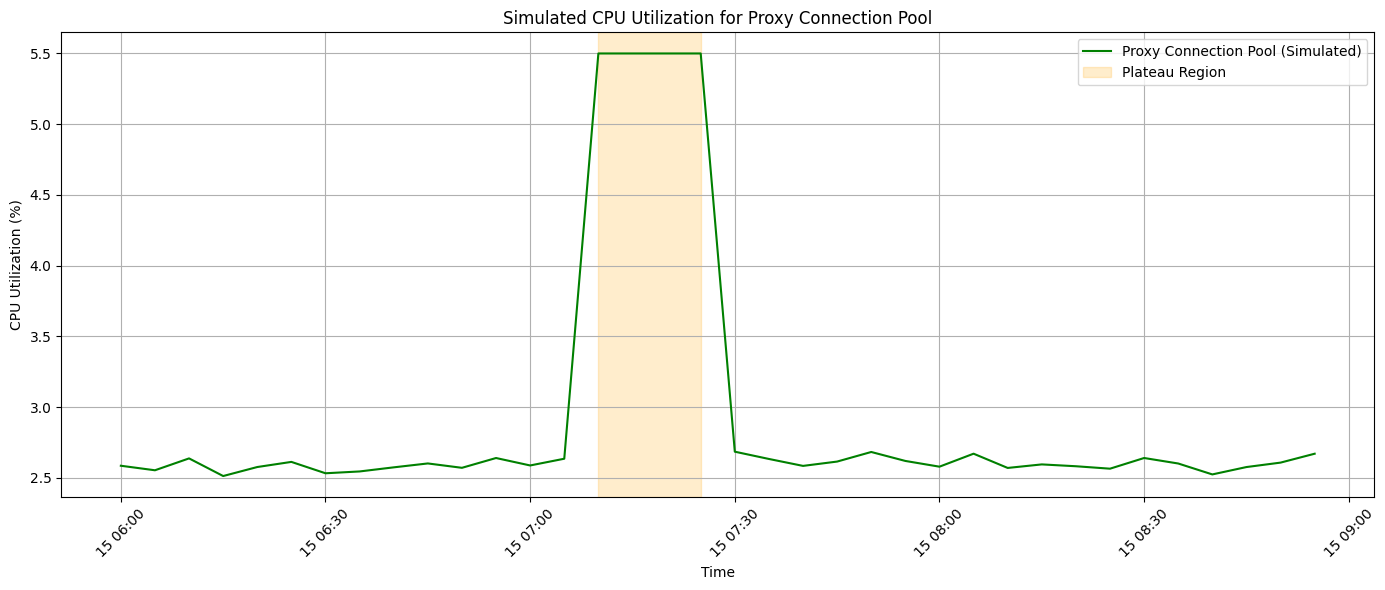
\includegraphics[width=0.75\linewidth]{images/image7.png}
    \caption{Simulated CPU Utilization for RDS Instance Using Proxy Connection Pool on 15 June 2025. The orange-shaded region between 03:07:00 and 03:07:00 represents a plateau period where CPU usage stabilizes at approximately 5.5\%, simulating load handling through a connection pool.}
    \label{fig:proxy_rds_cpu}
\end{figure}

\begin{figure}[H]
    \centering
    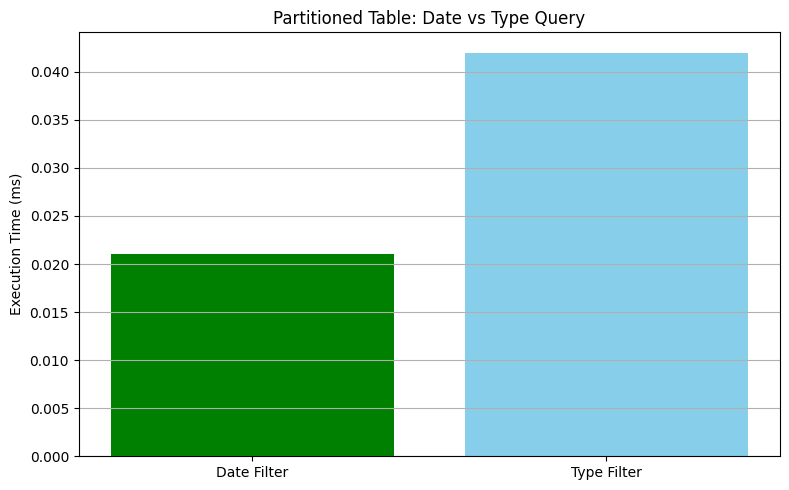
\includegraphics[width=0.75\linewidth]{images/image8.png}
    \caption{Performance metrics comparison between Proxy Connection and Direct RDS Connection. The Proxy setup demonstrates significantly lower connection time and latency, while achieving higher throughput (TPS), suggesting better efficiency under load.}
    \label{fig:performance_comparison}
\end{figure}


\subsection{Discussion}
A data-driven comparison between direct client-to-database interactions and an intermediary layer that uses Proxy Connection Pooling is provided by the analysis done on AWS RDS performance metrics. Plotting the connection data and CPU utilization trends over time reveals various important insights and performance constraints.

\paragraph{CPU Utilization & Load Behavior}
As shown in Fig. 1, the base CPU utilization for the primary RDS instance stays within a stable range (~2.5–2.7) during normal operation. However, the graph in Fig. 6 highlights a notable CPU spike between 07:10 and 07:25 UTC under direct connection usage, corresponding to a surge in client requests. This indicates potential resource stress when sudden concurrency occurs, leading to latency or throttling risks.

By contrast, Fig. 7 illustrates the effect of introducing a proxy-based connection pool. During the same high-load window, CPU usage stabilizes into a plateau (~5.5) rather than spiking. This plateau demonstrates how connection pooling buffers incoming requests, flattening bursts and enabling the database to maintain predictable performance.

\paragraph{Connection Load Analysis}
Fig. 5 presents the number of active connections to a read replica, showing a burst around 03:40 that peaks near 50 connections. Without pooling, this load could overload the instance. However, connection pooling (as in Fig. 7) mitigates this behavior by multiplexing database sessions, effectively shielding the backend from such spike

\paragraph{Performance Metrics Comparison}
The benchmarking results (shown in Fig. 8) demonstrate clear benefits of using a proxy. Latency drops from ~1189 ms to ~823 ms, initial connection time improves drastically from over 1000 ms to ~118 ms, and TPS (Transactions Per Second) increases from ~84 to ~121. These improvements directly translate to enhanced responsiveness and throughput in real-world applications.

\paragraph{Partitioning for Query Optimization}
As outlined in Table III, partitioning the events table by event time results in a massive performance gain—reducing query execution time from 34.227 ms to just 0.021 ms. The optimization stems from partition pruning, which narrows the scope of data access. Instead of scanning the entire dataset, only the relevant partition is queried, significantly reducing I/O overhead. This approach is highly effective for time-series or log data queries.

\paragraph{Read Replica Behavior}
Fig. 4 captures CPU usage for a read replica, showing intermittent spikes (up to 25)T during likely read-intensive workloads. While replicas offload read traffic from the primary, they can still be overwhelmed without additional safeguards like query throttling or pooling. These spikes may correspond to report generation, backup tasks, or analytics, implying the need for targeted traffic management.

\begin{table}[htbp]
\centering
\small
\begin{tabular}{|p{2.4cm}|p{2.4cm}|p{2.4cm}|}
\hline
\textbf{Scaling Technique} & \textbf{Use Case Scenario} \\
\hline
Vertical Scaling & OLTP, small/medium workloads \\
\hline
Read Replicas & Read-heavy, analytics, reporting \\
\hline
Partitioning & Large datasets, time-series data \\
\hline
Connection Pooling & High-concurrency, microservices \\
\hline
Custom Sharding & Global, high-write, massive scale \\
\hline
Kubernetes-Based Scaling & Cloud-native, dynamic, automation \\
\hline
Hybrid/Elastic Scaling & Mixed workloads, variable demand \\
\hline
\end{tabular}
\caption{use Case Table collection}
\label{tab:postgresql_research_summary}
\end{table}

\section{Conclusion}
Among all of the techniques evaluated, Connection Pooling provides us the most immediate and cost-efficient benefit\cite{b13}. As demonstrated in our benchmarks (Fig. 8), it reduces the initial connection time by ~88\% (from 1022.5 ms to 118.6 ms), decreases the latency by ~30\% (from 1189.8 ms to 823.2 ms), and increases the TPS by ~44\% (from 84.05 to 121.44). These improvements validate its role as a protective buffer layer that mitigates CPU spikes (from 6.5\%+ peaks in Fig. 6 to a stable 5.5\% plateau in Fig. 7), They efficiently absorbing high-concurrency workloads without modifying the underlying RDS infrastructure \cite{b17}.

For read-heavy scenarios, Read Replicas effectively offload traffic from the primary instance \cite{b19}, \cite{b20}. As seen in the (Fig. 4,) read operations causes the CPU spikes exceeding 25\%, indicating that replicas can  also absorb peak read demand. However, careful orchestration is needed to prevent connection storms, such as the sudden surge to ~50\% connections observed in Fig. 5, which ofter lead's to temporary bottlenecks.

\begin{thebibliography}{26}
\bibitem{b1} H. C. S. Perera et al., "Database Scaling on Kubernetes," in 2021 3rd International Conference on Advancements in Computing (ICAC), Colombo, Sri Lanka, 2021, pp. 258--263.
\bibitem{b2} A. Kumar et al., "Horizontal vs. Vertical Scaling in Modern Database Systems: A Comparative Analysis of Performance and Cost Trade-Offs," International Journal of Computer Engineering and Technology (IJCET), vol. 15, no. 5, pp. 514--524, Sep.--Oct. 2024.
\bibitem{b3} Codecademy, "Database Scaling Strategies," 2022. [Online]. Available: https://www.codecademy.com/article/database-scaling-strategies
\bibitem{b4} DZone, "The Ultimate Database Scaling Cheatsheet," 2024. [Online]. Available: https://dzone.com/articles/ultimate-database-scaling-cheatsheet
\bibitem{b5} A. Sengar, "Top 10 Database Scaling Techniques," LinkedIn, May 2025. [Online]. Available: https://www.linkedin.com/pulse/top-10-database-scaling-techniques-we-engineer-should-avadhesh-sengar-3jizc
\bibitem{b6} K. Yerkade, "Maximizing Performance: Best Practices for Database Scaling," DEV, Oct. 2024. [Online]. Available: https://dev.to/kaustubhyerkade/maximizing-performance-best-practices-for-database-scaling-2fkn
\bibitem{b7} Q. Wang, "PostgreSQL Database Performance Optimization," Bachelor's Thesis, Business Information Technology, Marlevo Software Oy, 2011. [Online]. Available: https://www.theseus.fi/bitstream/handle/10024/29980/ThesisReport\_Qiang\_Wang.pdf
\bibitem{b8} Anonymous, "PostgreSQL as a Multi-Model Database," Master's Thesis, East Carolina University, 2019. [Online]. Available: https://thescholarship.ecu.edu/items/ddb7ccb4-513f-4719-8a58-b2e0301a504b
\bibitem{b9} A. Lakshman and P. Malik, "Cassandra: A Decentralized Structured Storage System," ACM SIGOPS Oper. Syst. Rev., vol. 44, no. 2, pp. 35--40, Apr. 2010.
\bibitem{b10} A. Cruz et al., "The Choice of Scaling Technique Matters for Classification Performance," arXiv, Dec. 26, 2022. [Online]. Available: https://arxiv.org/abs/2212.12343
\bibitem{b11} S. Kumar, "Measurement and Scaling Techniques in Research Methodology," SSRN, Aug. 18, 2022. [Online]. Available: https://papers.ssrn.com/sol3/papers.cfm?abstract\_id=4178691
\bibitem{b12} S. Zhong and M. Rigger, "Scaling Automated Database System Testing," in Proc. Conference, New York, NY, USA: ACM, 2018, pp. 1--14.
\bibitem{b13} N. A. N. Sobri et al., "A Study of Database Connection Pool in Microservice Architecture," Journal of Open Innovation: Technology, Market, and Complexity, vol. 6, no. 2, article 1094, 2022.
\bibitem{b14} U. Cubukcu et al., "Citus: Distributed PostgreSQL for Data-Intensive Applications," in Proc. 2021 International Conference on Management of Data (SIGMOD '21), 2021, pp. 2490--2502.
\bibitem{b15} J. Dean and S. Ghemawat, "MapReduce: Simplified Data Processing on Large Clusters," in Proc. OSDI 2004, 2004, pp. 137--150.
\bibitem{b16} M. Zaharia et al., "Resilient Distributed Datasets: A Fault-Tolerant Abstraction for In-Memory Cluster Computing," in Proc. USENIX NSDI 2012, 2012, pp. 15--28.
\bibitem{b17} M. Armbrust et al., "A View of Cloud Computing," Commun. ACM, vol. 53, no. 4, pp. 50--58, Apr. 2010.
\bibitem{b18} C. Mohan et al., "Aries: A Transaction Recovery Method Supporting Fine-Granularity Locking and Partial Rollbacks Using Write-Ahead Logging," ACM Trans. Database Syst., vol. 17, no. 1, pp. 94--162, Mar. 1992.
\bibitem{b19} Y. Lin et al., "Middleware Based Data Replication Providing Snapshot Isolation," in Proc. ACM SIGMOD 2005, 2005, pp. 419--430.
\bibitem{b20} S. Elnikety, W. Zwaenepoel, and F. Pedone, "Database Replication Using Generalized Snapshot Isolation," in Proc. IEEE SRDS 2006, 2006, pp. 73--84.
\bibitem{b21} D. J. DeWitt and J. Gray, "Parallel Database Systems: The Future of High Performance Database Systems," Commun. ACM, vol. 35, no. 6, pp. 85--98, Jun. 1992.
\bibitem{b22} A. Pavlo, C. Curino, and S. Zdonik, "Skew-aware Automatic Database Partitioning in Shared-nothing, OLTP Systems," in Proc. ACM SIGMOD 2012, 2012, pp. 61--72.
\bibitem{b23} S. Idreos, M. L. Kersten, and S. Manegold, "Database Cracking: Towards Auto-tuning Database Kernels," in Proc. IEEE ICDE 2007, 2007, pp. 323--332.
\bibitem{b24} J. Gray, "Notes on Database Operating Systems," in Operating Systems: An Advanced Course, vol. 60, Springer, 1978, pp. 393--481.
\bibitem{b25} S. Das, D. Agrawal, and A. El Abbadi, "ElasTraS: An Elastic Transactional Data Store in the Cloud," in Proc. USENIX HotCloud 2009, 2009.
\bibitem{b26} E. Brewer, "CAP Twelve Years Later: How the 'Rules' Have Changed," Computer, vol. 45, no. 2, pp. 23--29, Feb. 2012.
\end{thebibliography}
\vspace{12pt}

\end{document}